%&pdflatex
\section{Impostazione degli utenti}
Linux è un sistema \textit{multi-utente}. Esiste, in ogni sistema Linux, un \textit{utente amministratore} con privilegi massimi sul sistema chiamato \texttt{root}. Il prossimo passo è impostare la password dell'account amministratore \texttt{root} (Figura \vref{fig:root-password}).

\begin{figure}[ht]
	\centering
	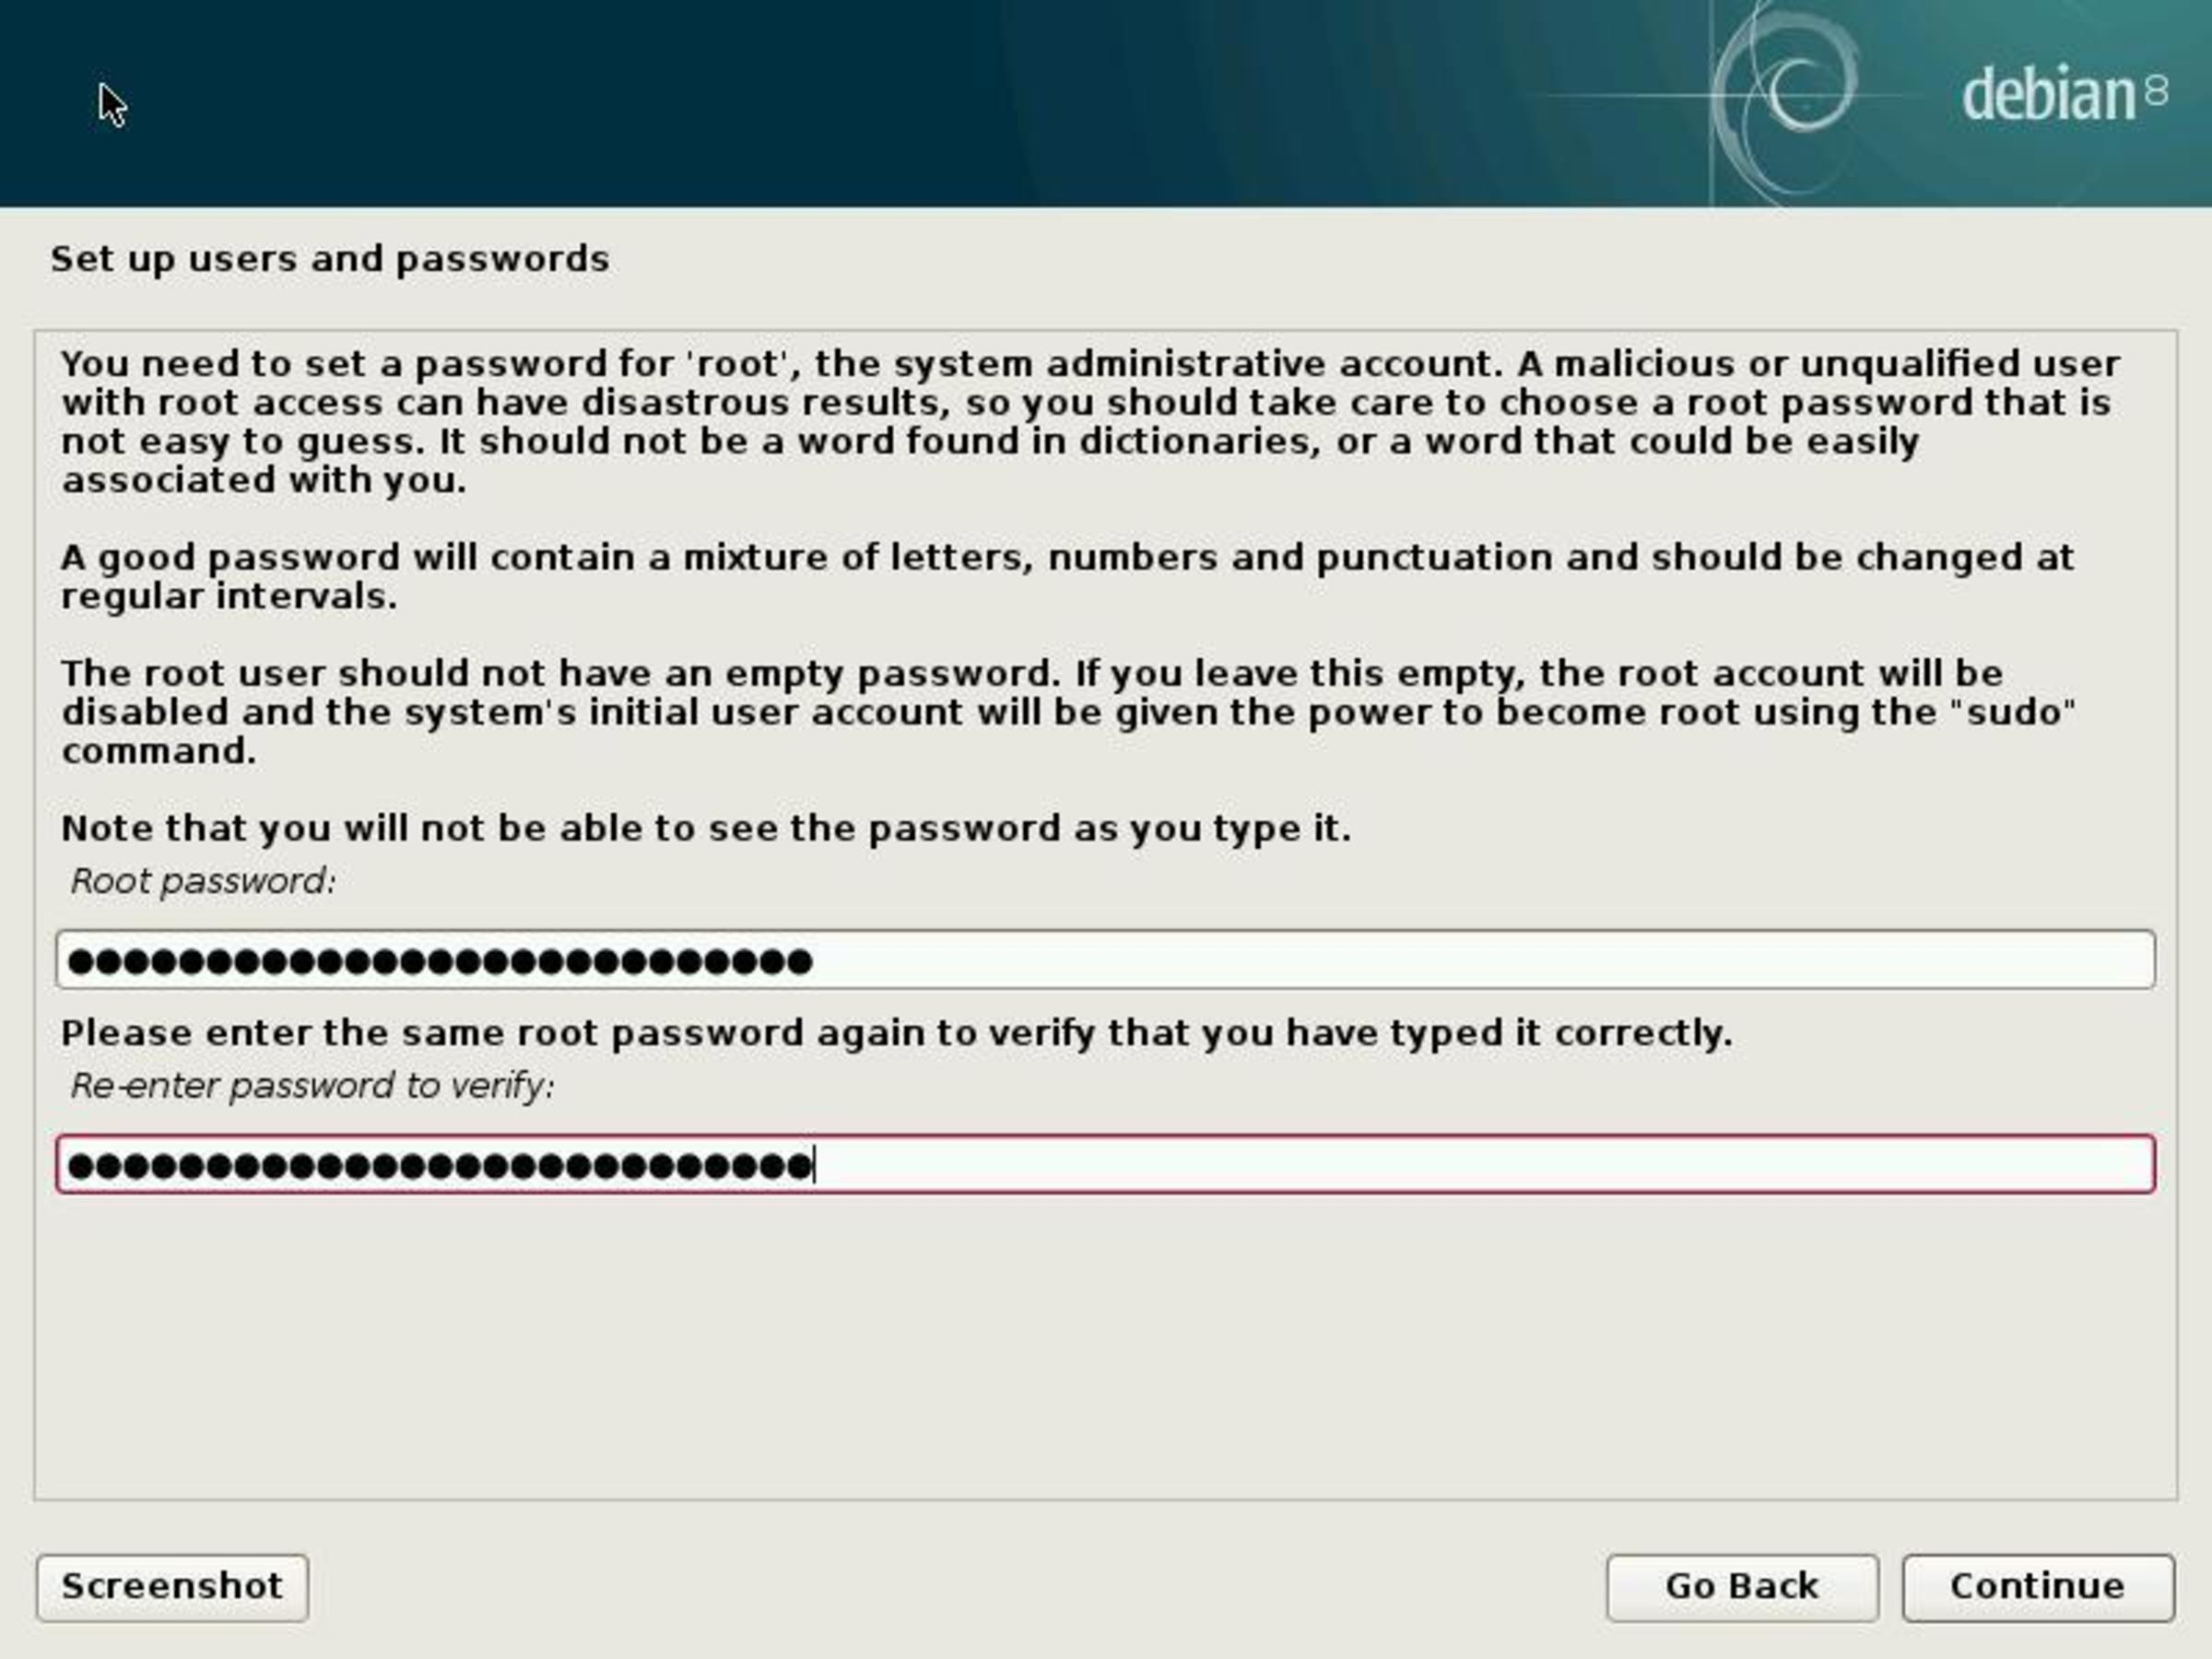
\includegraphics[resolution=600]{root-password}
	\caption{Impostazione della password dell'account \texttt{root}}
	\label{fig:root-password}
\end{figure}

La password non dovrebbe essere troppo semplice da indovinare e dovrebbe essere sufficientemente lunga e sicura. Bisogna tenere presente che una persona che ha accesso come \texttt{root} a un sistema Linux può anche, ad esempio, cancellare tutti i file (sistema operativo compreso) presenti nel disco!

Successivamente, ci verrà chiesto di creare un nuovo \textit{utente standard}. Essendo pericoloso usare \texttt{root} per le attività quotidiane (se si scarica uno \textit{script} contenente \texttt{rm -rf -{}-no-preserve-root /} e si esegue utilizzando l'account \texttt{root} l'intero disco viene cancellato), viene solitamente creato un account personale con privilegi limitati: nel momento in cui sono necessari privilegi amministrativi, sarà sempre possibile accedere temporaneamente come \texttt{root}. Il primo passo è scegliere un \textit{nome completo}. Questo, dovrebbe essere il nome reale dell'utente (ad esempio \texttt{Niccolò Scatena}). Successivamente, sarà chiesto di inserire un \textit{username} che verrà usato per il login: l'username deve essere tutto minuscolo (ad esempio \texttt{speedjack}). Infine, bisogna scegliere la password del nuovo account (in genere, diversa da quella di \texttt{root}).
